\documentclass[article,shortnames]{jss}

%%%%%%%%%%%%%%%%%%%%%%%%%%%%%%
%% declarations for jss.cls %%%%%%%%%%%%%%%%%%%%%%%%%%%%%%%%%%%%%%%%%%
%%%%%%%%%%%%%%%%%%%%%%%%%%%%%%

%% almost as usual
\author{Lindsay Rutter\\Iowa State University \And 
        Susan VanderPlas\\Iowa State University \And
        Di Cook\\Monash University\And
        Michelle Graham\\Iowa State University}
\title{\pkg{ggenealogy}: An \proglang{R} Package for Visualizing Genealogical Data}

%% for pretty printing and a nice hypersummary also set:
\Plainauthor{Lindsay Rutter, Susan VanderPlas, Di Cook} %% comma-separated
\Plaintitle{ggenealogy: An R Package for Visualizing Genealogical Data} %% without formatting
\Shorttitle{\pkg{ggenealogy}: An \proglang{R} Package for Visualizing Genealogical Data} %% a short title (if necessary)

%% an abstract and keywords
\Abstract{
  This paper introduces \pkg{ggenealogy} (\citealt{ggen}), a developing \proglang{R} package that provides tools for searching through genealogical data, generating basic statistics on their graphical structures using parent and child connections, and displaying the results. It is possible to draw the genealogy in relation to variables related to the nodes, and to determine and display the shortest path distances between genetic lines. Production of pairwise distance matrices and genealogical diagrams constrained on generation are also available in the visualization toolkit. The software is being tested on datasets with milestone cultivars of soybean (\citealt{soybean}) and barley varieties [2], as well as on data from the \citealt{mgp}, a database of the academic genealogy of mathematicians. It is currently available on the Comprehensive R Archive Network.}

\Keywords{genealogy, data visualization, statistical graphics, exploratory data analysis, interactive, \proglang{R}}
\Plainkeywords{genealogy, data visualization, statistical graphics, exploratory data analysis, interactive, R} %% without formatting
%% at least one keyword must be supplied

%% publication information
%% NOTE: Typically, this can be left commented and will be filled out by the technical editor
%% \Volume{50}
%% \Issue{9}
%% \Month{June}
%% \Year{2012}
%% \Submitdate{2012-06-04}
%% \Acceptdate{2012-06-04}

%% The address of (at least) one author should be given
%% in the following format:
\Address{
  Lindsay Rutter\\
  Bioinformatics and Computational Biology Program\\
  Iowa State University\\
  2014 Molecular Biology Building\\
  Ames, IA, 50011, United States of America\\
  E-mail: \email{lrutter@iastate.edu}\\
  URL: \url{https://github.com/lrutter/}\\

  Susan VanderPlas\\
  Department of Statistics\\
  Iowa State University\\
  2413 Snedecor Hall\\
  Ames, IA, 50011, United States of America\\
  E-mail: \email{srvanderplas@gmail.com}\\
  URL: \url{https://github.com/srvanderplas/}\\
  
  Di Cook\\
  Department of Econometrics and Business Statistics\\
  Monash University\\
  E869 Menzies Building\\
  20 Chancellors Walk\\
  Clayton, VIC 3800, Australia\\
  E-mail: \email{dicook@monash.edu}\\
  URL: \url{https://github.com/dicook/}\\

  Michelle Graham\\
  USDA-Agriculture Research Service, Corn, Insects and Crop Genetics Research Unit\\
  Department of Agronomy, Iowa State University\\
  1575 Agronomy Building\\
  Ames, IA, 50011, United States of America\\
  E-mail: \email{magraham@iastate.edu}
}

%% It is also possible to add a telephone and fax number
%% before the e-mail in the following format:
%% Telephone: +43/512/507-7103
%% Fax: +43/512/507-2851

%% for those who use Sweave please include the following line (with % symbols):
%% need no \usepackage{Sweave.sty}

%% end of declarations %%%%%%%%%%%%%%%%%%%%%%%%%%%%%%%%%%%%%%%%%%%%%%%

\begin{document}

%% include your article here, just as usual
%% Note that you should use the \pkg{}, \proglang{} and \code{} commands.

%% \section[About Java]{About \proglang{Java}}
%% Note: If there is markup in \(sub)section, then it has to be escape as above.

\section{Introduction}

Genealogy is the study of the parent-child relationships. By tracing through lineages of groups of individuals, the history of features that have been modified over time can be studied. Comparative geneticists, computational biologists, and bioinformaticians commonly use these tools to better understand the historical changes that caused novel and desirable traits to arise in lineages. For example, in crops, desirable modifications could include an increase in protein yield or an increase in disease resistance. However, there are also times when lineages of detrimental traits are analyzed, such as to determine the origin of hazardous traits in rapidly-evolving viruses.

Furthermore, genealogical relationships can be applied outside of a strict biological sense, an example being the \citealt{mgp}, which maintains the family lineage of academic mathematicians, with documentation of doctoral advisors, doctoral students, and graduation years of all mathematicians in academia. Such family lineages allow us to understand the position of one member in the larger historical picture, and to accurately preserve past relationships for the knowledge of future generations.

In all these examples, the data structures containing the genealogical relationships can be represented visually. Access to various types of visual plots and diagrams of the lineage can allow scientists and others to more efficiently and accurately explore an otherwise complicated data structure. We introduce here a developing visualization toolkit that is intended to assist users in their exploration and analysis of genealogical relationships. In this paper, we will demonstrate some of the main features of this software package, and summarize any novelty that such features may provide users, using an example lineage dataset of soybean cultivars (\citealt{soybean}).

\section{Available Software}

Publishing in the open source \proglang{R} statistical programming language allows for tools to be distributed and modified at ease, encourages cross-platform collaboration, and provides a foundation for effective and aesthetic data visualization from the grammar of graphics. There are several useful \proglang{R} packages that offer tools for analyzing and visualizing genealogical datasets. Here, we introduce these packages, and emphasize the new features that \proglang{ggenealogy} brings to this collection of work.

The \proglang{R} package \proglang{pedigree} is named after the standardized chart used by genealogists to study human family lines, and sometimes used to select breeding of animals, such as show dogs (\citealt{ped}). The package uses a similar data input type as \proglang{ggenealogy}, namely a data frame for parent and child labels. While it does provide tools to perform methods on the data set, such as rapidly determining the generation count for each member in the pedigree, it does not provide any visualization tools.

Another \proglang{R} package called \proglang{kinship2} does produce basic pedigree charts, one from the package vignette of which is provided as an example in Figure \ref{fig:kinshipFig} (\citealt{kin}). This pedigree chart adheres to the standard notations used for visualizing genealogical structures. Even though doing so creates powerful charts that can be applied across many applications, it cannot provide unequivocal information in situations where inter-generational cross-breeding occurs, as is often the case in agronomical genealogical lineages. We demonstrate how the standardized pedigree charts in the \proglang{kinship2} package generate ambiguous results in such scenarios by superimposing a hypothetical inter-generational cross-breeding case in Figure \ref{fig:kinshipFig}. We then later illustrate how new plotting tools in the \proglang{ggenealogy} package resolve this previously unaddressed area in Figure \ref{fig:Lee}.

In addition, popular graph drawing software such as \proglang{GraphViz} and \proglang{Cytoscape} can be used to visualize genealogical structures, as is shown in Figure \ref{fig:Graph} (\citealt{graphvizCit}, \citealt{cytoscapeCit}). These programs allow for visualizations of graphs, which are defined as objects with sets of nodes and edges, where nodes cannot be repeated. However, as is described in Figure \ref{fig:Lee}, for certain genealogical datasets to be non-ambiguously displayed (as is described in ), Hence, as is the case with the aforementioned \proglang{R} packages, these popular software also cannot

\begin{figure}[h]
    \centering
    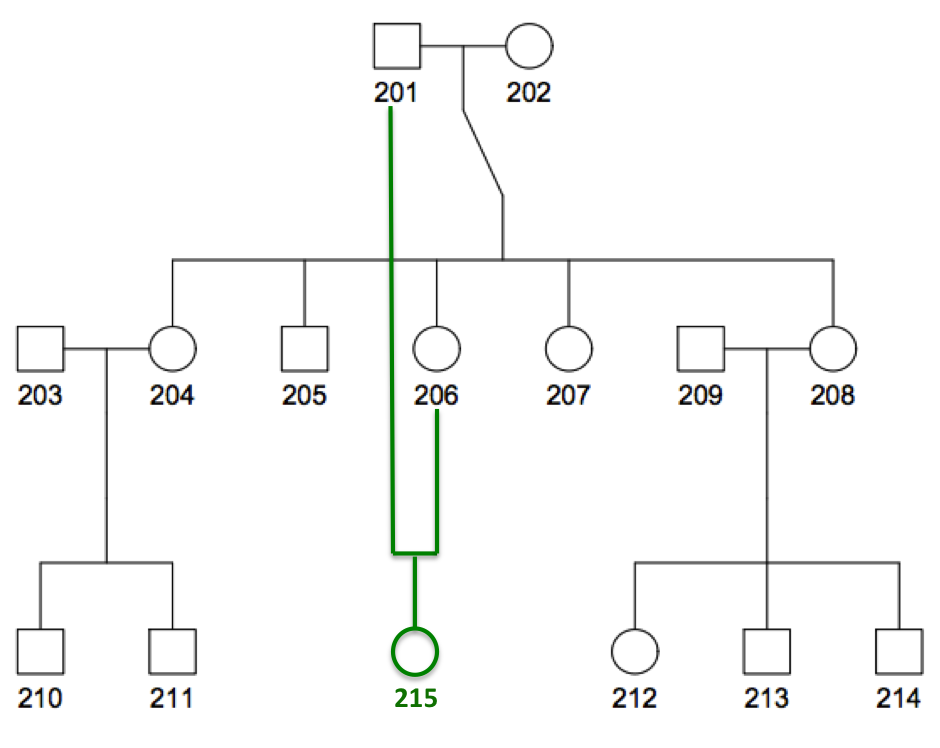
\includegraphics[width=0.65\textwidth]{kinshipFig}
    \caption{Example pedigree chart output from the \proglang{kinship2} package. A standardized set of symbols are used to represent males with squares and females with circles. Parents are connected to each other by horizontal lines, and to their children by vertical lines. Siblings are connected by horizontal sibship lines. Each generation is defined by its position on the vertical axis, with the first generation containing individuals 201 and 202. We superimposed green-highlighted individual 215 and its corresponding connections onto the pedigree chart for explanatory purposes. Its parents are individuals 201 and 206, which are from generations one and two, respectively, and have a parent-child relationship themselves. As an offspring of a parent-child relationship, individual 215 is both a second generation and third generation individual. Hence, individual 215 should be displayed in both generational positions on the vertical axis. However, standard pedigree tools only allow for an individual to be displayed once. As a result, in cases where inter-generational cross-breading occurs, such as in agronomical applications, standardized tools for visualizing genealogical information cannot non-ambiguously portray the genealogical dataset.}
    \label{fig:kinshipFig}
\end{figure}

\begin{figure}[h]
    \centering
    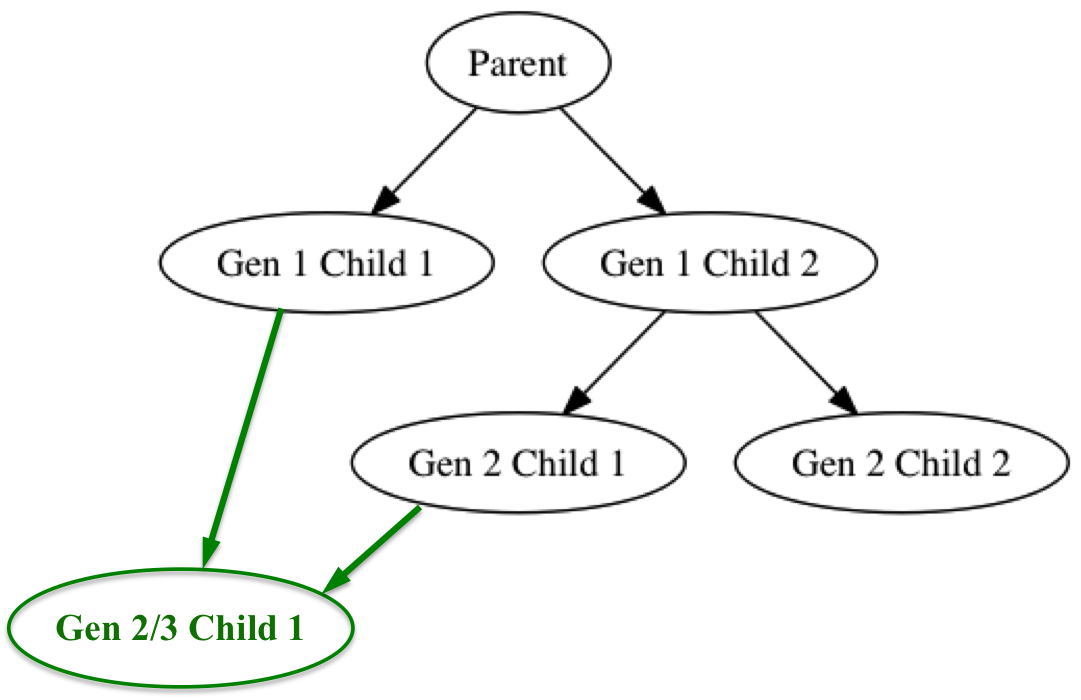
\includegraphics[width=0.6\textwidth]{Graph}
    \caption{Example genealogical display using popular software like \proglang{GraphViz} and \proglang{Cytoscape}. The generation count of an individual node is constrained by its position on the vertical axis. As was shown in Figure \ref{fig:kinshipFig}, here too we superimpose a green node that has parents from the first and second generations. As an offspring of parents from two different generations, this green node is both a second generation and third generation individual of the original parent. Hence, it should be displayed in both corresponding generation positions on the vertical axis. However, standard graph visualization tools only allow for a given ode to be displayed once. As a result, this green node must be ambiguously positioned as either a second or third generation individual; here, it is positioned as a third generation individual.}
    \label{fig:Graph}
\end{figure}

\section{Soybean Genealogy Dataset}

The \proglang{ggenealogy} package comes with two example datasets, one comprises a soybean genealogy and the other comprises an academic statistician genealogy. We will introduce both example datasets in this paper to demonstrate some of the tools available in the software. We start with the soybean genealogy, which is available in a data frame structure with 412 rows, each representing a direct parent-child relationship between a pair of soybean varieties. In total, there are 230 unique soybean varieties in the dataset. These data were collected from field trials, genetic studies, and United States Department of Agriculture (USDA) bulletins, and date as early as the first decade of the 1900s. They also contain information on the developmental years, as well as the copy number variants, single nucleotide polymorphisms, protein content, and yield, of each of the soybeans.

In this context, the software could ideally be used by bioinformaticians, geneticists, and agronomists who wish to study how soybean varieties are related. By referencing the visualization of the genealogical tree, these scientists may better understand genetic testing results - in this particular dataset, in terms of copy number variants, single nucleotide polymorphisms, protein content, and yield - and use that knowledge in future breeding sessions.

\section{Generating a Graphical Object}

Most functions in the software package require an input parameter of a graph structure. Therefore, as a preprocessing step, we must first convert our original data frame structure into a graph structure. Below, we read in the \proglang{R} data file \code{sbGeneal} that is included in the package as a sample data set of soybean genealogy.

\begin{CodeChunk}
\begin{CodeInput}
R> library("ggenealogy")
R> data(sbGeneal)
R> str(sbGeneal)
\end{CodeInput}
\begin{CodeOutput}
'data.frame':	412 obs. of  5 variables:
 $ child       : chr  "5601T" "Adams" "A.K." "A.K. (Harrow)" ...
 $ year        : num  1981 1948 1910 1912 1968 ...
 $ yield       : int  NA 2734 NA 2665 NA 2981 2887 2817 NA NA ...
 $ year.imputed: logi  TRUE FALSE TRUE FALSE FALSE FALSE ...
 $ parent      : chr  "Hutcheson" "Dunfield" NA "A.K." ...
\end{CodeOutput}
\end{CodeChunk}

We now convert it into an \pkg{igraph} object (\citealt{igraph}) \code{sbIG} using the function \code{dfToIG()}.

\begin{CodeChunk}
\begin{CodeInput}
R> sbIG <- dfToIG(sbGeneal)
R> sbIG
\end{CodeInput}
\begin{CodeOutput}
IGRAPH UNW- 230 340 -- 
+ attr: name (v/c), weight (e/n)
+ edges (vertex names):
 [1] 5601T    --Hutcheson        Adams    --Dunfield        
 [3] A.K.     --A.K. (Harrow)    Altona   --Flambeau        
 [5] Amcor    --Amsoy 71         Adams    --Amsoy           
 [7] Amsoy 71 --C1253            Anderson --Lincoln         
 [9] Bay      --York             Bedford  --Forrest         
[11] Beeson   --Kent             Blackhawk--Richland        
[13] Bonus    --C1266R           Bradley  --J74-39          
[15] Bragg    --Jackson          Bragg    --Bragg x D60-7965
+ ... omitted several edges
\end{CodeOutput}
\end{CodeChunk}

There are many statistics about the \code{sbGeneal} genealogical dataset that we may wish to know that cannot easily be obtained through images and tables. The package function \code{getBasicStatistics()} can be called, using the \code{sbIG} object as input. This will return a list of common graph theoretical measurements regarding the genealogical graph structure. For instance, is the whole structure connected? If not, how many separated components does it contain? In addition to these statistics, the \code{getBasicStatistics()} function will also return the number of nodes, the number of edges, the average path length, the graph diameter, and other graph theoretical information.

\begin{CodeChunk}
\begin{CodeInput}
R> getBasicStatistics(sbIG)
\end{CodeInput}
\begin{CodeOutput}
$isConnected
[1] FALSE

$numComponents
[1] 11

$avePathLength
[1] 5.333746

$graphDiameter
[1] 13

$numNodes
[1] 230

$numEdges
[1] 340

$logN
[1] 5.438079
\end{CodeOutput}
\end{CodeChunk}

\section{Plotting a Shortest Path}

As this data set deals with soy bean lineages, it may be useful for agronomists to track how two varieties are related to each other via parent-child relationships. Then, any dramatic changes in protein yield, SNP varieties, and other measures of interest between the two varieties can be traced across their genetic timeline, and pinpointed to certain varieties within their historical lineage. The \pkg{ggenealogy} software allows users to select two varieties of interest, and determine the shortest pathway of parent-child relationships between them, using the \code{getPath()} function. This will return a list path that contains the variety names and their years in the path.

\begin{CodeChunk}
\begin{CodeInput}
R> pathTN <- getPath("Tokyo", "Narow", sbIG, sbGeneal)
R> pathTN
\end{CodeInput}
\begin{CodeOutput}
$pathVertices
[1] "Tokyo"    "Volstate" "Jackson"  "R66-873"  "Narow"   

$yearVertices
[1] "1907"   "1942"   "1954.5" "1971.5" "1985" 
\end{CodeOutput}
\end{CodeChunk}

The returned path object can then be plotted using the \code{plotPath()} function, as demonstrated below.

\begin{Code}
R> plotPath(pathTN)
\end{Code}

\begin{figure}[h]
    \centering
    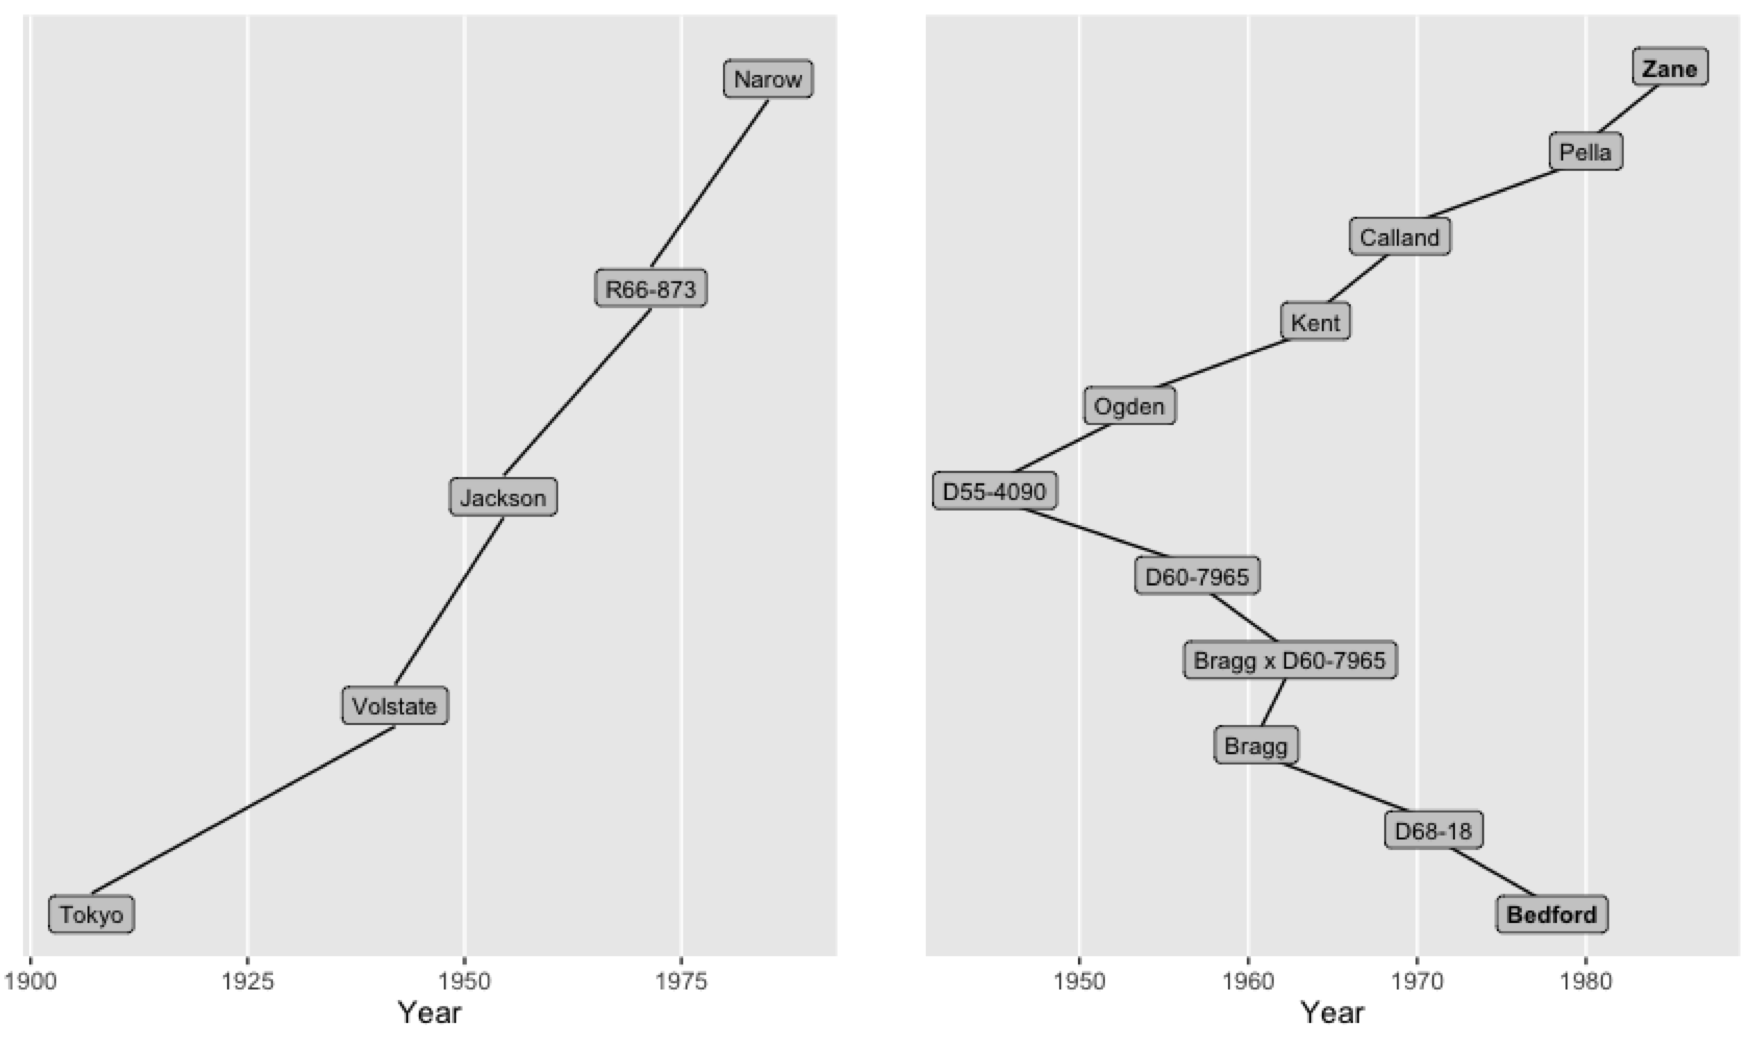
\includegraphics[width=\textwidth]{pathTNZB}
    \caption{Left: The shortest path between varieties Tokyo and Narow is strictly composed of a unidirectional sequence of parent-child relationships. Right: The shortest path between varieties Zane and Bedford is not strictly composed of unidirectional parent-child relationships, but have a cousin-like relationship.}
    \label{fig:pathTNZB}
\end{figure}

This produces a visual that informs users of all the varieties involved in the shortest path between the two varieties of interest, see left half of Figure \ref{fig:pathTNZB}. In this plot, the years of all varieties involved in the path are indicated on the horizontal axis, while the vertical axis has no meaning other than to simply to display the labels evenly spaced vertically. The shortest path between varieties \code{Tokyo} and \code{Narow} is composed of a unidirectional series of parent-child relationships, with \code{Tokyo} as the starting ancestor in the early 1900s, \code{Narow} as the most recent descendent in the mid 1980s, and three varieties in between.

Next, we can run the same set of functions on a different pair of varieties. First, a call to the \pkg{ggenealogy} function \code{getYear()} indicates that variety \code{Bedford} was developed in 1978 and variety \code{Zane} in 1985.

\begin{CodeChunk}
\begin{CodeInput}
R> getYear("Bedford", sbGeneal)
\end{CodeInput}
\begin{CodeOutput}
[1] 1978
\end{CodeOutput}
\begin{CodeInput}
R> getYear("Zane", sbGeneal)
\end{CodeInput}
\begin{CodeOutput}
[1] 1985
\end{CodeOutput}
\end{CodeChunk}

We can then create a plot showing the shortest path between these two varieties of interest.

\begin{Code}
R> pathBZ <- getPath("Bedford", "Zane", sbIG, sbGeneal)
R> plotPath(pathBZ)
\end{Code}

The resulting plot (right half of Figure \ref{fig:pathTNZB}) allows us to quickly determine that \code{Bedford} is not a parent, grandparent, or any great grandparent of \code{Zane}. Instead, we see that these two varieties are not related through a unidirectional parent-child lineage, but have a cousin-like relationship. The oldest common ancestor between \code{Zane} and \code{Bedford} is the variety \code{D55-4090}, which was developed in the mid 1940s.

Furthermore, as determined by the figure, for both \code{Zane} and \code{Bedford}, there are four varieties of unidirectional parent-child relationships between each of them and their common ancestor \code{D55-4090}. Hence, any parameter of interest that differentiates \code{Zane} and \code{Bedford} (protein yield, disease resistance, etc.) can also be examined across these two separate lineage histories.

\section{Superimposing Shortest Path on Tree}

Now that we can create path objects, we may wish to know how those paths are positioned in comparison to the genealogical lineage of the entire data structure. For instance, of the documented soybean cultivar lineage varieties, where does the shortest path between two varieties of interest exist? Are these two varieties comparatively older compared to the overall data structure? Are they newer? Or, do they span the entire structure, and represent two extreme ends of documented time points?

There is a function available in the \pkg{ggenealogy} package \code{plotPathOnAll()} that can allow users to quickly visualize their path of interest superimposed over all varieties and edges present in the whole data structure. Here we will produce a plot of the previously-determined shortest path between varieties \code{Tokyo} and \code{Narow} across the entire dataset:

\begin{Code}
R> plotAllImage <- plotPathOnAll(pathTN, sbGeneal, sbIG, binVector = 1:3,
  pathColor = "red")
R> plotAllImage ggplot2::theme(axis.text = ggplot2::element_text(size = 12), axis.title = ggplot2::element_text(size = 12))
R> plotAllImage <- plotPathOnAll(path = path, geneal = sbGeneal, ig = sbIG
  binVector = sample(1:3), edgeCol = "gray84", pathEdgeCol = "blue", nodeSize
  = 1, pathNodeSize = 3)
\end{Code}

\begin{figure}%[h]
    \centering
    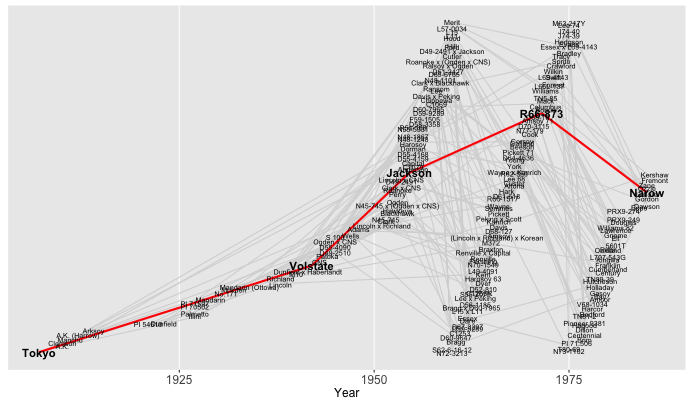
\includegraphics[width=\textwidth]{plotTNBin3}
    \caption{The shortest path between Tokyo and Narow, superimposed over the data structure, using a bin size of 3.}
    \label{fig:plotTNBin3}
\end{figure}

While the first three explicit parameters to the function \code{plotPathOnAll()} have been introduced earlier in this paper, the fourth parameter (\code{binVector}) requires some explanation. The motivation of the \code{plotPathOnAll()} is to write variety text labels on a plot, with the center of each variety label constricted on the horizontal axis to its developmental year. As is the case for the plots before, the vertical axis has no meaning other than providing a plotting area in which to draw the text labels. Unfortunately, for large datasets, this motivation can be a difficult task because the text labels of the varieties can overlap if they are assigned a similar y coordinate, have a similar year (x coordinate), and have labels with large numbers of characters (width of x coordinate).

For each variety, the x coordinate (year) and width of the x coordinate (text label width) cannot be altered, as they provide useful information. However, for each variety, the y coordinate is arbitrary. Hence, in an attempt to mitigate text overlapping, the \code{plotPathOnAll()} does not randomly assign the y coordinate. Instead, it allows users to partially control the y coordinates with a user-determined number of bins (\code{binVector}).

If the user determines to produce a plot using three bins, as in the example code above, then the varieties are all grouped into three bins based on their years of development. In other words, there will be bin 1 (the ``oldest bin") which includes one-third of the total number of varieties all with the oldest developmental years, bin 2 (the ``middle bin"), and bin 3 (the ``youngest bin").

Then, in order to decrease text overlap, the consecutively increasing y-axis coordinates are alternatively assigned to the three bins (For example: bin 1, then bin 2, then bin 3, then bin 1, then bin 2, then bin 3, ...) repeatedly until all varieties are accounted for. This algorithm means that for any pair of varieties within a given bin constrained to those years on the horizontal axis, there are exactly two other varieties placed between them vertically on the y-axis that come from the two other bins 1 constrained to a different set of year values on the horizontal axis.

Hence, in the code above, the user selected a \code{binVector} value of three, and a \code{plotColor} of red, which produces the plot in Figure \ref{fig:plotTNBin3}. We see that edges not on the path of interest are thin and gray by default, whereas edges on the path of interest are bolded and red. We also see that varieties in the path of interest are boldfaced by default.

The plot presents useful information: We immediately gather that the path of interest between does span most of the years of the data structure. In fact, \code{Tokyo} appears to be the oldest variety present in the dataset, and \code{Narow} appears to be one of the youngest varieties. We can also determine that the vast majority of varieties appear to have development years between 1950 and 1970.

However, this plot has significant empty spaces between the noticeably distinct bins, whereas almost all text labels are overlapping, thereby decreasing their readability. To force some variety text labels into these spaces, the user may consider using a larger number of bins. Hence, we next examine a bin size of 6:

\begin{Code}
R> plotAllImage <- plotPathOnAll(pathTN, sbGeneal, sbIG, binVector = 1:6,
  pathEdgeCol = "seagreen2", nodeSize = 1, pathNodeSize = 3)
\end{Code}

\begin{figure}%[h]
    \centering
    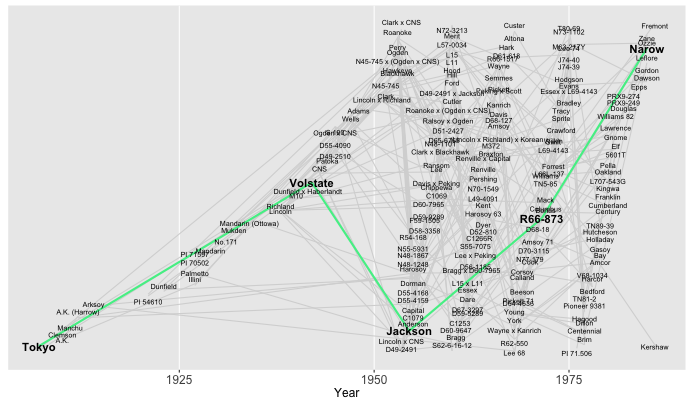
\includegraphics[width=\textwidth]{plotTNBin6}
    \caption{The shortest path between Tokyo and Narow, superimposed over the data structure, using a bin size of 6.}
    \label{fig:plotTNBin6}
\end{figure}

This similar code now outputs the plot shown in Figure \ref{fig:plotTNBin6}. We can immediately see that this plot more successfully mitigates text variety label overlap than the previous plot in \ref{fig:plotTNBin3}. We can also confirm what we saw in the previous plot that indeed most varieties have development years between 1950 and 1970, and any textual overlap is confined to this range of years.

\section{Future Directions: Fine-tuning Superimposition}

This visualization tool is suitable as part of a data exploration phase, but not for any users seeking publication quality plots due to the remaining textual overlap. We continue to work towards further reducing this textual overlap, although it is impossible to guarantee no textual overlap, especially with larger datasets with dense subgroups of varieties having similar years.

As such, we plan to add a feature to the \pkg{ggenealogy} package that allows users to manually fine-tune the plot they deem best after examining various bin sizes. For example, after comparing several bin sizes (1-12) on the current soy bean data set, we determined that the bin size of 6 produced minimal textual overlap, as seen in \ref{fig:plotTNBin6}.

However, there still remained one dozen cases of partial textual overlap. As an example, the labels of \code{Crawford} (1974) and \code{Swift} (1973) overlap at just below the vertical midpoint of the plot. The proposed function would allow users to hardcode the label of either variety and manually assign it to a new vertical coordinate. For instance, a user might select \code{Swift} and slightly decrease its vertical coordinate so that it is drawn halfway between \code{Crawford} and \code{Bradley}.

If the user sequentially fine-tuned the vertical positions of overlapping text labels for the small fraction of labels that remained overlapped after the automated function, and if they monitored the progress by visually inspecting updated plots until there were no more overlaps, then the plot could be used in presentations and publications.

\section{Plotting Ancestors and Descendants by Generation}

The most novel visual tool in \pkg{ggenealogy}, \code{plotAncDes()}, allows users to view the ancestors and descendants of a given variety. The inputted variety is highlighted in the center of the plot, ancestors are displayed to the left of the center, and descendants to the right of the center. The further from the center, the larger the number of generations that particular ancestor/descendant is from the centered variety of interest.

This particular \pkg{ggenealogy} tool is unique because most available graphical software only consider simple graphs, with no repeated nodes. However, in some genealogical lineage datasets, some varieties must be repeated if they are to be visualized by generation counts. This was found to be the case in the soy bean dataset.

As an example, we will create a plot of the ancestors and descendants of the variety \code{Lee}. We specify that the maximum number of ancestor and descendant generations are both 6, and that the text of the variety of interest is highlighted in blue:

\begin{Code}
R> plotAncDes("Lee", sbGeneal, mAnc = 6, mDes = 6, vCol = "blue")
\end{Code}

\begin{figure}%[h]
    \centering
    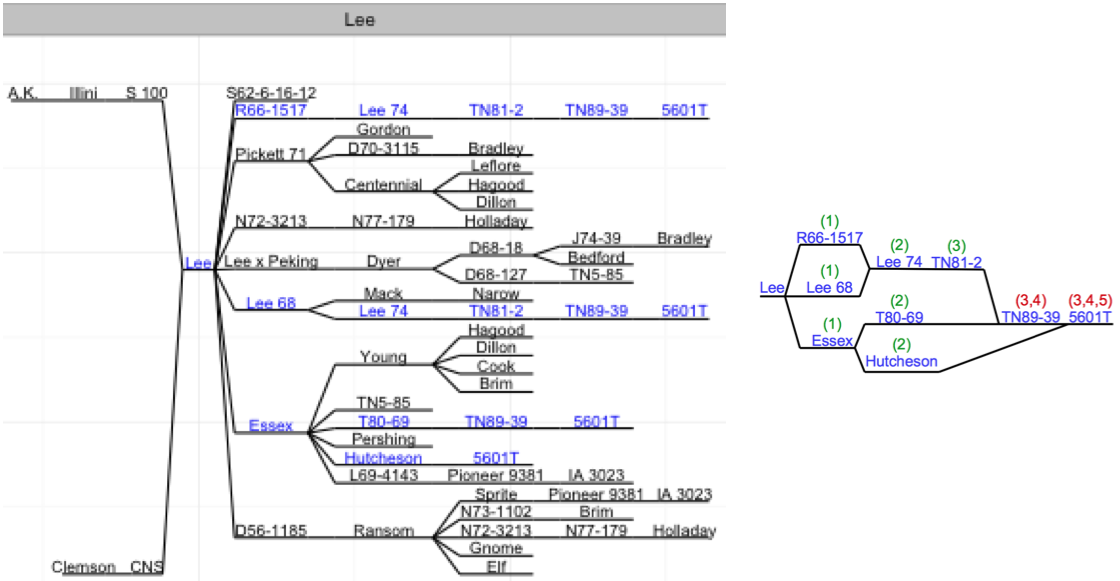
\includegraphics[width=\textwidth]{Lee}
    \caption{Left: All varieties within three generations of ancestors and five generations of descendants of the variety Lee are shown. The generation distance from the center variety is neatly displayed in this graph; the larger the generation distance from the center variety, the further left (for ancestors) or right (for descendants). For explanation purposes, all paths between Lee and 5601T are highlighted in blue. We see that 5601T appears four times in the plot, which is a unique and novel requirement provided by ggenealogy. Right: The paths that are highlighted in blue in the left plot from ggenealogy are shown here again, only now nodes cannot be repeated. We unsuccessfully try to constrain the horizontal position of the nodes by generation count, as was accomplished by the ggenealogy plot, without repeating nodes. The parenthetical number above each node represents the set of generation counts that node is away from the center node Lee; green ones indicate that the node could be successfully placed in one horizontal position, but red ones indicate that the node could not be successfully placed in only one horizontal position. Hence, without allowing nodes to repeat, this data information cannot be presented as it is in the ggenealogy graph on the left, and this is a current limitation in other currently-available graphical software that ggenealogy can now provide.}
    \label{fig:Lee}
\end{figure}

This generates the plot we see in the left side of Figure \ref{fig:Lee}. We notice that \code{Lee} has 3 generations of ancestors and 5 generations of descendants. However, we also notice that some varieties are repeated in the plot. For example, the variety \code{5601T} is represented four times - once as a third generation descendant of \code{Lee}, once as a fourth generation descendant of \code{Lee}, and twice as a fifth generation descendant of \code{Lee}.

This happens because there are various paths between \code{Lee} and \code{5601T} (see the right side of Figure \ref{fig:Lee}). Hence, if we are to present all ancestors and descendants of \code{Lee} - while constricting the horizontal axis to generational distance from \code{Lee} - then varieties like \code{5601T} must occur more than once in the plot.

One of the main motivations in developing the \code{plotAncDes()} function was an inability to find other similar software (\citealt{ape}) that could produce such a plot, where repeated nodes were permitted, see right side of Figure \ref{fig:Lee} for additional explanation. The \code{plotAncDes()} function generates plots that have increased readability, as it is relatively easy to compare how far varieties are from the center to obtain an idea of generational distance.

\section{Plotting Distance Matrix}

It may also be of interest to generate matrices where the colors indicates a variable (such as the degree of the shortest path) between all pairwise combinations of inputted varieties. The package \pkg{ggenealogy} also provides a function \code{plotDegMatrix()} for that purpose.

Here we generate a distance matrix for a set of 10 varieties, setting the x-label and y-label as ``Variety" and the legend label as ``Degree". Syntax from the \pkg{ggplot2} package (\citealt{ggplot2}) can be appended to the \code{plotDegMatrix()} function. In this example, we add \pkg{ggplot2} functionality to specify that pairs with small degrees are white, while those with large degrees are dark green, as well as to specify the label size of the legend title and text:

\begin{Code}
>R varieties <- c("Brim", "Bedford", "Calland", "Dillon", "Hood", "Narow",
  "Pella", "Tokyo", "Young", "Zane")
>R plotDegMatrix(varieties, sbIG, sbGeneal, "Variety", "Variety", "Degree") +
  ggplot2::scale_fill_continuous(low = "white", high = "darkgreen") +
  ggplot2::theme(legend.title = ggplot2::element_text(size = 15),
  legend.text = ggplot2::element_text(size = 15))
\end{Code}

\begin{figure}[h]
    \centering
    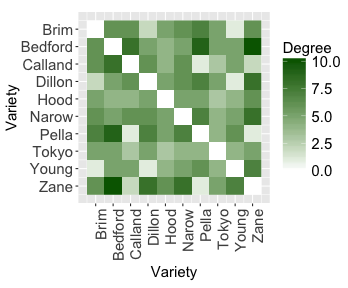
\includegraphics[width=0.5\textwidth]{degMatrix}
    \caption{The shortest path degree matrix between ten varieties of interest.}
    \label{fig:degMatrix}
\end{figure}

This creates the plot in Figure \ref{fig:degMatrix}. We see that the degree of the shortest path between varieties \code{Bedford} and \code{Zane} is 10, which is consistent with what we saw earlier in Figure \ref{fig:pathTNZB}. However, we now also see that 10 may be a comparatively large degree in this same dataset.

\section{Academic Genealogy of Statisticians}

In addition to the soybean genealogy, the \proglang{ggenealogy} package also comes with an academic genealogy of statisticians. To develop this later dataset, we contacted the Mathematics Genealogy Project, a web-based database for the genealogy of academic mathematicians. This database, which currently contains almost 200,000 entries, is a service of the North Dakota State University Department of Mathematics and the American Mathematical Society. The Mathematics Genealogy Project contact provided us a Structured Query Language (SQL) export, and we used PostgreSQL to query the database (\citealt{psql}).

Each entry in the database contained 26 variables pertaining to an individual who received a graduate-level academic degree in statistics. One of these variables was called ``msc" (Mathematics Subject Classification), and we selected only those entries that contained a value of 62 for this variable (coded as ``Statistics"). Furthermore, we only retained those entries that, if they contained an advisor, then that advisor was also in the field ``Statistics". This process resulted in 8995 entries, which we reduced to 8166 entries by removing duplicate entries. With the final data frame of 8995 entries, we only maintained 6 of the variables.

This process resulted in the second example dataset provided in the \proglang{ggenealogy} package. This dataset is structured as a data frame that contains 8166 rows, each of which corresponds to a parent-child relationship, where both the child and the parent received postbaccalaureate degrees in statistics, and the parent was the academic advisor to the child. The columns of the dataset provide information about the year the child obtained the degree, the country and school from which the child obtained the degree, and the thesis title of the degree awarded to the child.

\begin{CodeChunk}
\begin{CodeInput}
R> data(statGeneal)
R> dim(statGeneal)
\end{CodeInput}
\begin{CodeOutput}
[1] 8166    6
\end{CodeOutput}
\begin{CodeInput}
R> colnames(statGeneal)
\end{CodeInput}
\begin{CodeOutput}
[1] "child"   "parent"  "year"    "country" "school"  "thesis"
\end{CodeOutput}
\end{CodeChunk}

%\section{Plotting Ancestors and Descendants by Generation}

This second example dataset of academic genealogy is of a slightly different structure than the first example dataset of agronomical genealogy, because each child no longer requires exactly two parents. The ability to plot ancestors and descendants by generation was demonstrated on the agronomical genealogy in Figure \ref{fig:Lee}. As we believe this is the most novel plotting tool in the \proglang{ggenealogy} package, we can test it again here using the academic genealogy.

We can determine which academic statistician in this \code{statGeneal} dataset has the largest number of descendants. To do so, we create a vector \code{indVec} that contains the names of all individuals (whether child or parent) in the dataset. We then use the \proglang{dplyr} package to apply the ggenealogy function \code{getDescendants} on each individual in the \code{indVec} vector (\citealt{dplyr}). We set the parameter \code{gen} to a conservatively large value of 100 as this dataset is unlikely to have any individuals with more than 100 generations of descendants.

We then create a table to examine all values of descendant counts observed in the dataset, along with the number of individuals who had each of those values of descendant counts. Of the 8166 individuals in this dataset, 6252 of them have zero descendants, 322 of them have one descendant, and 145 of them have two descendants. There are only 17 individuals who have more than 30 descendants, and there is one individual who has the largest value of 159 descendants. We determine that this individual is the prominent British statistician Sir David Cox, who is known for the Box-Cox transformation and Cox processes, as well as for mentoring many younger researchers who later became notable statisticians themselves.

\begin{CodeChunk}
\begin{CodeInput}
>R library(dplyr)
>R indVec <- unique(c(statGeneal$child, statGeneal$parent))
>R indVec <- indVec[which(indVec != "", )]
>R dFunc <- function(var) nrow(getDescendants(var, statGeneal, gen = 100))
>R numDesc <- sapply(indVec, dFunc)
>R table(numDesc)
\end{CodeInput}
\begin{CodeOutput}
numDesc
   0    1    2    3    4    5    6    7    8    9   10   11   12   13   14 
6252  322  145   88   58   36   31   22   23   14   17   13   14    9    9 
  15   16   17   18   19   20   21   22   23   24   25   26   27   29   30 
   6    4    3    2    5    7    5    3    3    2    2    6    1    1    3 
  34   37   38   40   41   44   45   48   49   61   62   75   77   84  159 
   2    1    1    1    1    1    1    1    2    1    1    1    1    1    1
\end{CodeOutput}
\begin{CodeInput}
R> which(numDesc == 159)
\end{CodeInput}
\begin{CodeOutput}
David Cox 
     1980
\end{CodeOutput}
\end{CodeChunk}

We can now visualize how these 159 descedants are related to Sir David Cox by plotting parent-child relationships, with generation count constricted on the horizontal axis, similar to what we performed in Figure \ref{fig:Lee}. We create this in Figure \ref{fig:dCox} using the code below.

\begin{CodeInput}
R> plotAncDes("David Cox", statGeneal, mAnc = 6, mDes = 6, vCol = "blue")
\end{CodeInput}

\begin{figure}%[h]
    \centering
    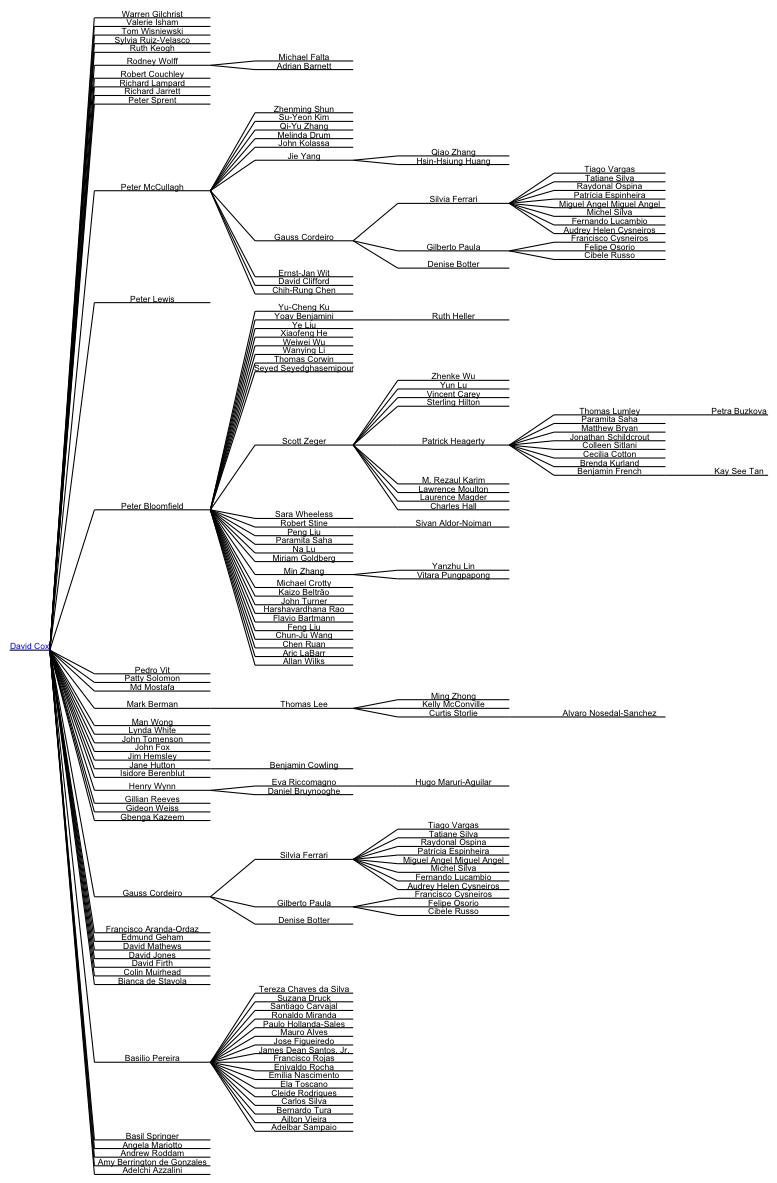
\includegraphics[width=\textwidth]{dCox.png}
    \caption{The 159 academic descendants of Sir David Cox.}
    \label{fig:dCox}
\end{figure}

We see from Figure \ref{fig:dCox} that Sir David Cox had 42 children, many of them becoming notable statisticians, such as Basilio Pereira, Valerie Isham, Gauss Cordeiro, Peter McCullagh, and Henry Wynn. The child of his who produced the most children of his own was Peter Bloomfield, who has 26 children and 49 descendants. In total, Sir David Cox has five generations of statistics students in this dataset.

\begin{CodeChunk}
\begin{CodeInput}
R> length(getChild("Peter Bloomfield", geneal))
\end{CodeInput}
\begin{CodeOutput}
[1] 26
\end{CodeOutput}
\begin{CodeInput}
R> nrow(getDescendants("Peter Bloomfield", geneal, gen = 100))
\end{CodeInput}
\begin{CodeOutput}
[1] 49
\end{CodeOutput}
\end{CodeChunk}

It would be insightful to examine a more detailed view of one of the longest strings of parent-child relationships between Sir David Cox and one of his fifth generation descendants. 

\begin{CodeChunk}
\begin{CodeInput}
R> statIG <- dfToIG(statGeneal)
R> pathCB <- getPath("David Cox", "Petra Buzkova", statIG, statGeneal, isDirected
  = FALSE)
R> plotPath(pathCB) + ggplot2::theme(axis.text = ggplot2::element_text(size
  = 12), axis.title = ggplot2::element_text(size = 12)) +
  ggplot2::scale_x_continuous(breaks = seq(1940, 2010, by = 10))
\end{CodeInput}
\end{CodeChunk}

\begin{figure}[h]
    \centering
    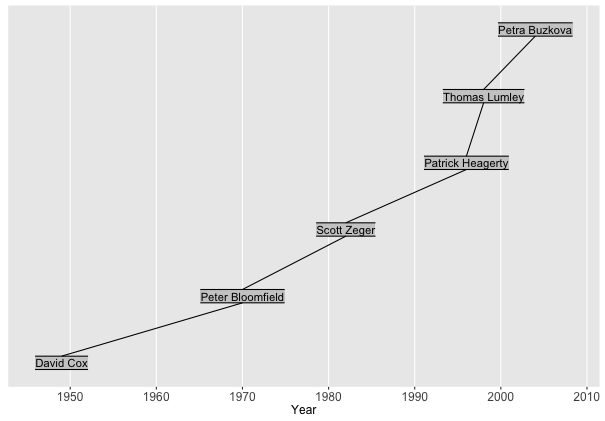
\includegraphics[width=\textwidth]{pathCB}
    \caption{The shortest path between Sir David Cox and Petra Buzkova is strictly composed of five unidirectional parent-child relationships that span about 55 years. We see that the time difference between when an advisor and student earned their degrees is not consistent across this path: The three statisticians who earned their degrees earliest in this path span more than about 30 years in degree aquisition, whereas the three statisticians who earned their degrees later in this path only span less than about 10 years in degree acquisition.}
    \label{fig:pathCB}
\end{figure}




\begin{figure}%[h]
    \centering
    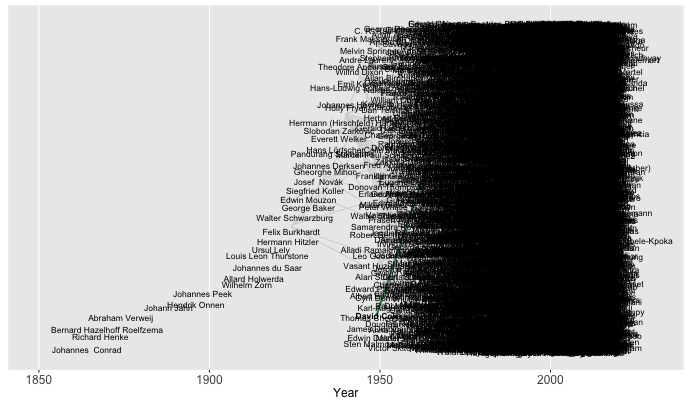
\includegraphics[width=\textwidth]{plotCBText}
    \caption{The shortest path between Tokyo and Narow, superimposed over the data structure, using a bin size of 6.}
    \label{fig:plotCBText}
\end{figure}

\begin{figure}%[h]
    \centering
    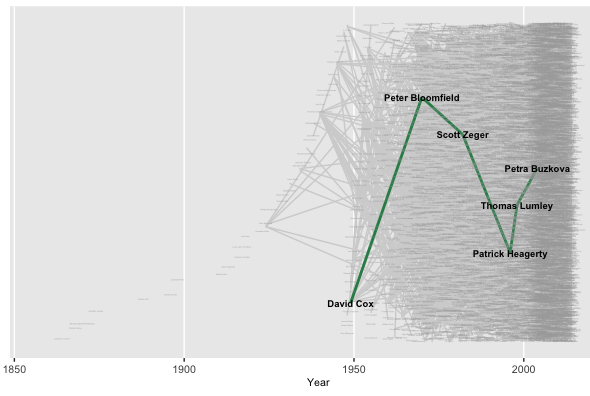
\includegraphics[width=\textwidth]{plotCBNoText}
    \caption{The shortest path between Tokyo and Narow, superimposed over the data structure, using a bin size of 6.}
    \label{fig:plotCBNoText}
\end{figure}

\section{Conclusions}

The \pkg{ggenealogy} package offers various plotting tools that can assist those studying genealogical lineages in the data exploration phases, as well as in preparing publication-suitable images. As each plot comes with its pros and cons, we recommended for users to explore several visualization tools. If users are simultaneously using similar packages, we in particular recommend using the \code{plotAncDes()} function. This plot allows users to view generation counts of a variety of interest in a manner that is not as readily available in similar software packages (\citealt{ape}).

\section{Future Avenues}

Incorporation of the Shiny application (\citealt{shiny}) would allow users to examine \pkg{ggenealogy} tools in a more interactive way. The reactive programming would save them the time of using command-line for each change of input as well as the inefficiency of rerunning code. We also look forward to testing this package on additional genealogical data sets (\citealt{mgp}). Exploring several datasets with our software will allow us to fix remaining bugs, and provide us further insight into how to make our tools available for a flexible set of data inputs.


\section*{Acknowledgments} % Lindsay added

The authors are grateful for the financial support from the United Soybean Board, North Central Soybean Research Program, the Iowa Soybean Association, the NSF Plant Genome Research Program (award number 0820642), and the USDA-Agricultural Research Service.

\bibliography{article}

\end{document}
